\documentclass{vldb}
\usepackage{graphicx}
\usepackage{balance, url,}  % for  \balance command ON LAST PAGE  (only there!)

\title{Probabilistic Consistency and Practical Non-strict Quorums}

\newdef{definition}{Definition}

\begin{document}

\maketitle

\noindent\textit{``All good ideas arrive by chance.''--Max Ernst}

\begin{abstract}


To lower the latency of read and write operations, operators of highly
available distributed data systems lower the required number of replicas
to be contacted per operation. This often results in non-overlapping
read and write replica sets, meaning the data store may return stale
data. However, modern eventually consistent quorum-based data stores
provide no guarantees on the staleness of data returned by these
so-called “non-strict” quorums.

In this work, we further develop the theory of probabilistic quorums
to provide meaningful bounds on the consistency of data items returned
by non-strict quorums of realistically-sized numbers of replicas. We
consider the staleness of data items across multiple versions and
across wall-clock time (taking anti-entropy processes into account),
including monotonic reads session guarantees. With this theory,
data system operators can determine the likelihood of various gradations
of staleness of returned data given a quorum system and then tune
their quorum selection to meet their desired application requirements.
We formulate an optimization of operation latency in terms of quorum
size given a staleness service level agreement and system load. We
subsequently implement these algorithms in an open source,
production-use distributed data system, Cassandra. Using this
implementation, we demonstrate how this theory can be practically
applied through both synthetic benchmarking and a sample deployment of
a social networking service running on our data system.

\end{abstract}

\section{Introduction}


Many of today's widely-deployed data storage solutions eschew ACID
guarantees in favor of BASE semantics, a large component of which is
the use of so-called eventual consistency of replicas.  In this model,
replicas are only guaranteed to eventually agree on the value of a
particular data item, and reads may return arbitrarily stale data.
The client-side semantics of this eventual consistency depend on
client access patterns~\cite{vogels-defs}, but, unless particular care
is taken, such as always contacting the same replica, the only
mechanism for ensuring strong consistency is to ensure overlapping
read and write quorums~\cite{dynamo}.

However, end-users today have come to expect undefined behavior
offering little to no insight into response consistency from their
eventually consistent data stores.  To achieve favorable performance,
users often employ \textit{non-strict or partial quorums}, in which
read and write sets are not guaranteed to overlap (given $n$ replicas
and read and write quorum sizes $r$ and $w$, $r+w \leq n$).  Modern
quorum-based scalable data systems such as Dynamo (and its open source
descendants Cassandra and Riak) provide no guarantees on the staleness
or consistency returned by non-strict quorums other than that the
system will ``eventually'' provide the right answer in the absence of
new writes.

In this paper, we prove that we can do better. Quorum-based data systems
can provide guarantees on the staleness of the data they provide. The
theory community has briefly explored the use of ``probabilistic
quorums'' to provide arbitrarily high probability of strong
consistency~\cite{prob-quorum}; in theory, these systems provide
excellent asymptotic behavior but are limited in practical
applicability due to their reliance on high replication factors.
Furthermore, in this theory, there is no guarantee on the recency of
data returned that is not the most recent version; with small $n$,
the probability of this happening is large---in the tens of percent.

In this work, we provide meaningful metrics for eventually consistent
data stores in the form of probabilistic bounded staleness.  By
relaxing the consistency guarantees from strong consistency to a
bounded-staleness model, we provide exponential improvements in the
probability of returning staler-than-promised data, resulting in
techniques that are useful at replication levels as seen in practice
($n<10$, and easily $n\leq3$).  One can easily predict the staleness
of his or her data (e.g., within 1 version with $70\%$ probability,
with 2 versions with $95\%$ probability, and so on).  From a
service-level agreement perspective, the system can minimize the
probability of returning staler-than-promised data to the order of
fractions of a percent.  It is much easier to write applications that
tolerate SLAs in the multiple ``nines'' reliability range than in the
high-tens-of-percent range.

Specifically, we provide algorithms and models for the staleness of a
data item across multiple versions and across real time and replica
propagation delay.  We can predict the probability of a request
falling within $k$ versions of the latest committed version after $t$
seconds have elapsed, for any $k$ and $t$, offering strongly
exponential improvements in the probability of returning
staler-than-promised data over the traditional literature.  We also
use these consistency measures to provide probabilistic guarantees on
monotonic reads, a form of session guarantees where reads are
guaranteed to return data items no older than what has been previously
read.

Using this theory, we can accurately provide read and write quorum
sizes ($w$,$r$,$n$) that optimize the performance of an operation on a
quorum-based data system given the desired staleness of a particular
partial quorum configuration.  Our models depend only on a model for
the latency of operations, which can be derived online and
continuously tuned.  We implement these algorithms on top of
Cassandra, a widely-deployed open source quorum-based distributed
data system, and demonstrating how to apply partial quorum theory in
practice.  We validate our new theory using several microbenchmarks
and synthetic workloads, then demonstrate the utility of staleness
measures in a Twitter clone with several thousand clients.

We make the following contributions in this paper:

\begin{itemize}

\item We further develop the theory of partial quorums to describe
  staleness probability metrics across both versions and time as well
  as probabilistic monotonic reads consistency.  This leads to
  exponentially lowered load per node and probability of
  inconsistency (Section~\ref{sec:theory}).

\item We employ this theory in optimizing read and write quorum sizes
  for minimum overall operational latency subject to a given
  service level agreement on the staleness of the data returned and
  the probability of further inconsistency (Section~\ref{sec:optimize}).

\item We implement this optimization layer and our algorithms in a
  modern distributed key-value store and demonstrate their utility in
  practice under both synthetic benchmarking and a web application
  workload (Section~\ref{sec:implement}).

\end{itemize}

\section{Background}

Write some stuff about quorum systems.


There are two main reasons to replicate data: durability and
scalability.  First, in the event of server failure, having stored the
data on multiple replicas allows end-users to continue to access the
data.  The replication factor in this case depends largely on the
relative ``importance'', or cost of losing the data.  Secondly, each
server has a maximum capacity, or number of requests that it can serve within a
given time period.  All else equal, replicating the data and
performing appropriate load-balancing lowers the load on each
individual server storing the data.

However, coordinating replicas has a cost; ensuring that all replicas
are up to date is expensive, but, as previously mentioned, giving up
ACID semantics lessens this cost.  By themselves, BASE semantics are
not immediately problematic: one cannot necessarily have all of
consistency, availability, and partition tolerance~\cite{cap-proof},
so, to achieve availability and partition tolerance, BASE systems give
up consistency.


\section{Probability and Partial Quorums}
\label{sec:theory}

SUMMARY

\subsection{Quorum Foundations: Theory}

Quorum systems have long been proposed as a replication strategy for
distributed data storage.  Informally, a strict quorum system defines
a set of sets of nodes in a distributed system with the property that
any two sets in the quorum system overlap (have non-empty
intersection).  When considering distributed get/put operations,
reading and writing to sets of nodes in a strict quorum system ensures
strong consistency in the absence of failures; the minimum sized
quorum defines its fault tolerance.  A simple example of a strict
quorum system is the majority quorum system, in which each quorum is
of size $\frac{N}{2}+1$.  However, the theory literature contains
numerous alternative quorum systems providing varying asymptotic
properties of capacity, scalability, and fault-tolerance, from
tree-quorums to grid-quorums.  Jim\'{e}nex-Peris et. al provide a
useful overview of these traditional, strict quorum
systems~\cite{quorums-alternative}.

Non-strict quorum systems are a natural extension of strict quorum
systems: at least two sets in a non-strict quorum system do not
overlap.  There are two relevant variants of non-strict quorum systems in
the literature: probabilistic quorum systems and k-quorums.

\textit{Probabilistic quorum systems} provide probabilistic guarantees
on the consistency of data returned by non-strict quorums.
Probabilistic quorums provide optimal (expected) load and fault
tolerance with an arbitrarily small probability of
inconsistency~\cite{prob-quorum}.  Intuitively, this is a consequence
of the Birthday Paradox: as the number of replicas increases, the
probability of non-overlap between any two subsets is quite low.
Given $n$ replicas and randomly chosen read and write quorums of sizes
$r$ and $w$, we can calculate the probability of the read quorum not
containing the value written by the write quorum.  The probability of
staleness is the number of quorums of size $r$ composed of nodes that
were not written to in the write quorum divided by the number of
possible quorums of size $r$:
\begin{equation}
\label{eq:prob-strict}
p_{stale}=\frac{{n-w \choose r}}{{n \choose r}}
\end{equation}
It is readily apparent that the probability of staleness is quite high
except for large values of $n$.  With $n=100$, $r=w=30$, $p_{stale} =
1.88 \times 10^{-6}$~\cite{nonstrict-availability}.  However, with
$n=3$, $r=w=1$, $p_{stale} = .\overline{6}$.  The asymptotics of these
systems are excellent---but only asymptotically.  To the best of our
knowledge, probabilistic quorums have only been used to study the
probability of strong consistency only.

\textit{$k$-quorum systems} provide strong (non-probabilistic)
guarantees that the partial quorum system will return a value that was
written within $k$ versions of the most recent
write~\cite{nonstrict-availability}.  In the single-writer scenario,
one can imagine a round-robin write scheduling scheme where each write
is sent to $\frac{n}{K}$ replicas such that each replica is no more
than $K$ versions out-of-date.  However, with multiple writers, one
loses the ordering properties that the single-writer was able to
control, and the best known algorithm for the pathological case
results in a lower bound of $(2n-1)(k-1)+n$ versions staleness~\cite{k-quorum-lb}.
Again, this prior work on $k$-quorums focused on purely deterministic
verion staleness.

This prior work has two properties with important implications for
practitioners.  First, existing theory treats quorums as static; a
write quorum is chosen and no other replicas in the system
subsequently learn about the value unless it is written again.  The
theory does not model anti-entropy processes.  Second, much of this
prior work assumes Byzantine failure.  If the description of prior
work seemed simplistic, it is largely because most of the literature
content addresses problems such as adversarial quorum selection and
scheduling.  In this work, we disregard both of these assumptions.  We
elaborate further in the next section.

\subsection{Quorum Foundations: Practice}
\label{sec:practice}

In practice, many distributed data management systems employ variable
quorum sizes. Amazon's Dynamo~\cite{dynamo} is the progenitor of a
class of eventually-consistent key-value stores that provide
quorum-style replication that includes Apache Cassandra, Basho's Riak,
and LinkedIn's Voldemort\footnote{Other BASE-style systems may employ
  master-slave replication, as in Apache HBase~\cite{hbase}.}.  In
this paper, we discuss Dynamo-style quorum systems, particularly
because we are not aware of any significally different production
quorum data systems.  However, with some work, we believe that other
systems can adopt our methodology.  Similarly, we focus on key-value
stores as the aforementioned systems provide some variant of key-value
architecture and do not provide full RDBMS semantics.  Quorum systems
may be employed in RDBMS replication, but, for simplicity, we describe
key-value stores here.

Dynamo-style quorum systems employ one quorum system per key,
typically maintaining the mapping of values to a set of nodes using a
consistent-hashing scheme or a centralized membership protocol. Each
node acts as a replica for multiple keys.  Client read and write
requests are sent to a proxy node in the key-value store and are
subsequently forwarded by the receiving node to all other nodes
assigned to that key as replicas.  The proxy node acknowledges
operation success when it has heard from a pre-defined number of
replicas.  Dynamo-style systems return guaranteed strongly consistent
data when $R+W > N$.  However, for improved latency, operators often
set $R+W \leq N$, typically $R=W=1$, as is the default for these
database systems (see Table TBD).

There are significant differences between data systems and the theory
describing quorum operation.  First, replication factors for
distributed data systems are relatively low.  Typical replication
factors are between one and three, however the literature has proposed
replication up to 10 (CITE CHAIN-REPLICATION).  Second, (in the
absence of failure), in Dynamo-style partial quorums, the number of
replicas that receive a write increases even after the operation
returns.  This is a simple version of anti-entropy.  Third, these
systems are often deployed in a trusted or semi-trusted computing
environment; there may be adversarial threats against data integrity
and denial-of-service attacks, but the underlying computing hardware
is non-adversarial. Within a controlled data center, the failure modes
are certainly reduced from the Byzantine case, and, despite its many
risks, the adversarial failures covered by prior theory appear
unlikely in emerging ``cloud computing'' environments.

\subsection{Assumptions}

These practical concerns guide the following theoretical
contributions.  Accordingly, we assume a quorum model where $w$ ($r$)
of $n$ replicas are randomly selected for each write (read) operation.
Unless otherwise noted, we consider fixed $w$ across multiple
operations.  We begin by considering a model without entropic
processes ($w$ is constant), then expand our model to consider
time-varying $w$. We consider a write ``committed'' once it has
reached $w$ replicas. We discuss further refinements to these
assumptions in Section \ref{sec:discussion}.

\subsection{Probabilistic $k$-quorums}

Probabilistic quorums allow us to determine the probability of
returning the most recent value written to the database, but it is
also useful to know the probability of returning a value within a
bounded number of versions.  Deterministic $k$-quorums provide
theoretical approaches to achieving this, however we can do better in
the presence of multiple writers by extending this theory to consider
probabilistic $k$-quorums.  In this model, we consider static write
quorums (no anti-entropy), but compose multiple write quorums to model the probable overlap of $k$ independent write sets.

\begin{definition}
A quorum system obeys \textit{probabilistic $k$-quorum consistency} if, with
probability $1-p_{staler}$, at least one value in any read quorum will
have been committed no later than $k$ versions after the latest committed
version when the read begins.
\end{definition}

Versions whose writes that are not yet committed (in-flight) may be
returned by a read in this formulation of probabilistic $k$-quorums
(see Figure \ref{fig:timelines}A).  The $k$-quorum literature defines these as $k$-regular semantics~\cite{nonstrict-availability}.

\begin{figure}
\centering
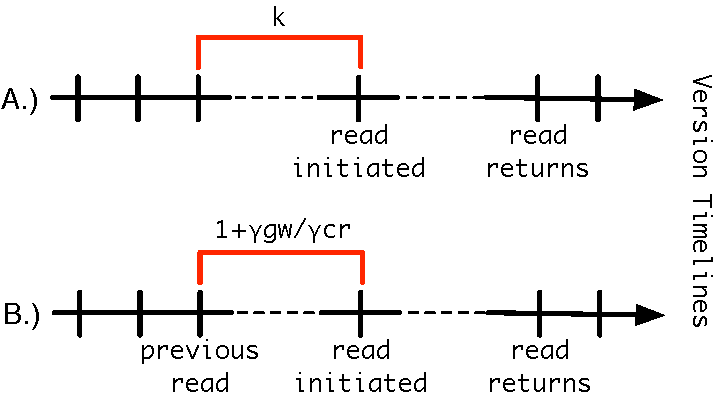
\includegraphics[width=\columnwidth]{figs/timelines.pdf}
\caption{Possible versions returned by read operations under
  probabilistic $k$-quorums (A) and monotonic reads (B). In
  $k$-consistency, the read operation will return a version no later
  than $k$ versions older than the last committed value when it
  started; more versions may be committed during the read and may be
  returned.  In monotonic reads consistency, the staleness depends on
  the number of versions committed since the time the client last
  completed a read.  This is determined by the proportion of client's
  reads to the number of writes committed to the object.}
\label{fig:timelines}
\end{figure}

The probability of returning a version of a key within $k$ versions is
equivalent to intersecting one of $k$ independent write
quorums\footnote{In the language of probabilistic quorums, we have
  constructed a probabilistic $k$-quorum from $k$ $\varepsilon$-quorum
  systems where $\varepsilon \leq \sqrt[k]{p_{staler}}$. This system
  has load $\geq \frac{1-\varepsilon^{\frac{1}{2k}}}{\sqrt{n}}$, an
  exponentially lower bound than a strict probabilistic quorum.  This
  follows immediately from~\cite[Corollary 3.12]{prob-quorum}}.
Quorums are chosen at random, so the probability of non-intersection
is simply Equation \ref{eq:prob-strict} exponentiated by $k$:

\begin{equation}
\label{eq:k-consistency}
p_s = \left(\frac{{n-w \choose r}}{{n \choose r}}\right)^k
\end{equation}

For the $n=3, r=w=1$ case, this means that the probability of
returning a version within $2$ versions is $.\overline{5}$, within $3$
versions $.\overline{703}$, and within $5$ versions $> .868$, and $10$
versions $>.98$.  With $n=3, r=1, w=2$ (alternatively, $r=2, w=1$),
these probabilities increase: $k=1 \rightarrow
.\overline{6}$, $k=2 \rightarrow .\overline{8}, k=5 \rightarrow >
.995$.

\subsection{Probabilistic Monotonic Reads}

With additional information, we can use probabilistic $k$-quorums to
predict whether a client will ever read stale data.  This property,
known as \textit{monotonic reads} consistency is a well-known session
guarantee~\cite{sessionguarantees}.

\begin{definition}
\label{def:prob-mr}
A quorum system obeys \textit{probabilistic monotonic reads consistency} if, with probaility at least $1-p_{staler}$, at
least one value in any read quorum the same version or a newer version
than the client's previously read value, where versions are defined
over the global commit ordering.
\end{definition}

To guarantee that a client sees monotonically increasing versions, it
can continue to contact the same replica~\cite{vogels-defs}, however
this is insufficient to guarantee strict monotonic reads (where the
client reads strictly newer data).  Definition~\ref{def:prob-mr} can
be adapted to acommodate strict monotonic reads (omitted for brevity).

We observe that monotonic reads is a special case of probabilistic
$k$-quorums where $k$ is determined by a client's rate of reads from a
data item ($\gamma_{cr}$) and the global, system-wide rate of writes
the same data item ($\gamma_{gw}$)\footnote{When constructed from $k$
  $\varepsilon$-consistent systems (as we have here), this consistency
  model has load $\geq
  \frac{(1-p_{staler}^{\frac{1}{2C}})}{\sqrt{n}}$, where
  $C=1+\frac{\gamma_{gw}}{\gamma_{cr}}$.}.  If we know these rates
exactly, the number of versions between client reads is
$\frac{\gamma_{gw}}{\gamma_{cr}}$, as shown in Figure
\ref{fig:timelines}B.  We can calculate the probability of
probabilistic monotonic reads as follows, effectively using Equation
\ref{eq:k-consistency} where $k=1+\frac{\gamma_{gw}}{\gamma_{cr}}$:

\begin{equation}
\label{eq:prob-mr}
p_{staler} = \left(\frac{{n-w \choose r}}{{n \choose r}}\right)^{1+\gamma_{gw}/\gamma_{cr}}
\end{equation}
For strict monotonic reads, exponentiate where $k=1+\frac{\gamma_{gw}}{\gamma_{cr}}$.

In practice, we may not know these exact rates, but, by measuring
their distribution, we can calculate an expected ratio that we can
integrate into these calculations.  However, by performing appropriate
admission control, operators can control these rates to achieve a
particular staleness target.

\subsection{Probabilistic $RT$-quorums}

Until now, we have considered only static write quorums.  However, as
we discussed in Section \ref{sec:practice}, modern quorum systems
propagate writes to all members of the quorum system for a given key.
This is commonly known as anti-entropy.  For generality, in this
section, we will discuss general anti-entropy models. However, we
explicitly model the Dynamo-style anti-entropy mechanism in Section
\ref{sec:dynamo-prop}.  Probabilistic $RT$-quorums model the
propagation of writes across wall-clock or real-world time such that
the set of replicas with a given version of the data (or later) grows
over time\footnote{Node failures shrink this set and can be
  incorporated into this model, but we do not consider them here.}.
We denote the probability density function describing the number of
replicas $\mathcal{W}$ that have a particular version $v$ (or a
version committed after $v$\footnote{We assume writes obey a total
  ordering. This can be accomplished using synchronized clocks (last
  writer wins) or with causal ordering and commutative merge
  functions~\cite{cops}.}) $t$ seconds after committing as
$p_l(\mathcal{W}, t)$.

\begin{definition}
A quorum system obeys \textit{probabilistic $RT$-quorum consistency}
if, with probability $1-p_{staler}$, at least one value in any read
quorum will either have been committed no greater than $t$ units of
time before the read began or will belong to an in-flight write.
\end{definition}

By definition, $p_l(c,0) = 1$ $\forall c \in [0, w]$.  Intuitively, at
commit time, $w$ replicas will have the value, so the probability that
zero to $w$ replicas have the value immediately after commit is
exactly $1$.  We can model the probability of probabilistic $RT$-consistency for an interval $t$ by summing the conditional probabilities of each possible $\mathcal{W}$:

\begin{equation}
p_{staler} = p_l(n, t)+\sum_{c\in[w, n)} \frac{{n-c \choose r}}{{n \choose r}} p_l(c, t)
\end{equation}

In practice, $p_l$ depends on the expected latency of operations and can be
approximated analytically (Section \ref{sec:dynamo-prop} or measured
online\footnote{For this reason, it is difficult to analytically
  determine the load of any probabilistically consistent system
  dependent on real-time operations.}.

\subsection{Probabilistic $\langle k, t
  \rangle$-quorum Consistency}

We can combine the previous models to combine both versioned and
real-time staleness metrics to answer questions of the following form:
what is the probability that a read will return a value no later than
$k$ versions old if the write committed no sooner than $t$ seconds
ago?

\begin{definition}
A quorum system obeys \textit{probabilistic $\langle k, t
  \rangle$-quorum consistency} if, with probability $1-p_{staler}$, at
least one value in any read quorum will have been committed no later
than $k$ versions after the latest committed version when the read
begins, provided the read begins $t$ units of time after the previous
$k$ versions commit.
\end{definition}

The definition of $p_{staler}$ follows from the prior definitions:

\begin{equation}
p_{staler} = \left(p_l(n, t)+\sum_{c\in[w, n)} \frac{{n-c \choose r}}{{n \choose r}} p_l(c, t)\right)^k
\end{equation}

In this equation, we assume the pathological case where the last $k$
writes all occurred at the same time.  This is not likely in practice,
so if we can determine the time since commit for the last $k$ writes,
we can improve this staleness bound by considering each quorum's $p_{stale}$ at $RT=t$ separately.

Note that the prior definitions of consistency are encapsulated by
probabilistic $\langle k, t \rangle$-quorum consistency. probabilistic
$k$-quorum consistency is simply probabilistic $\langle k, 0
\rangle$-quorum consistency, probabilistic monotonic reads consistency
is $\langle 1+\frac{\gamma_{gw}}{\gamma_{cr}}, 0 \rangle$-quorum
consistency, and $RT$-consistency is $\langle 0, RT \rangle$-quorum
consistency.

\subsection{Variable $w$}

\subsection{Typical Quorum Settings}

\section{Applied Theory and Refinements}
\label{sec:optimize}

\subsection{Operation Latency}

\label{sec:dynamo-prop}

Dynamo-style latency, assuming IID.  Alternative: measure empirically

Probability that $m$ of $n$ replicas respond to request at time $t$ given latency CDF $L$:

$$P_r(m, t, L) = (1-(L(t))^m)^{n \choose m}$$

$$r_t(r) = p_r(r, t, L_r)$$
$$w_t(r) = p_r(w, t, L_w)$$

Reads:

$$R_l(r) = \int_0^{\infty} r_t(r) l_r(t) dt$$

Writes

$$W_l(w) = \int_0^{\infty} w_t(w_{min}) l_r(t) dt$$



\subsection{Optimization Formulation}

We can use simple linear programming to determine what combination of
$r$ and $w$ (if any) minimizes latency while satisfying the system
constraints and user requirements.

Given $n$, desired $p$, $w_{min}$ (minimum committed $w$ before
returning), consistency model (with necessary parameters--$k$, $t$,
$\gamma_{cr}$, etc.), latency $L$, and the relative weighted
``importances'' of read and write latency, $c_r$ and $c_w$:

\begin{equation}
 \begin{array}{rl}
    \min        & R_l(r) +W_l(w) \\
    \mbox{s.t.} & p \ge p_s \\
                & w \ge w_{min}.
    \end{array}
\end{equation}

\subsection{Implications}
\label{sec:discussion}

Transactions

Variable $w$

Detection

\section{Experimental Evaluation}
\label{sec:implement}

\subsection{implementation}

\subsection{Synthetic Benchmarks}

\subsection{Twitter Clone}

\section{Conclusion}

\section*{Acknowledgements}

\balance

\bibliographystyle{abbrv}
\bibliography{ernst}

\end{document}

